\documentclass[simplex.tex]{subfiles}
% DO NOT INCLUDE PREAMBLES/PACKAGES HERE!!
% packages are inherited from preamble.tex; you can compile this on its own
\begin{document}
\subsection{FlashX}
%%% Jan
\begin{figure}[h!]
\begin{cframed}
\centering
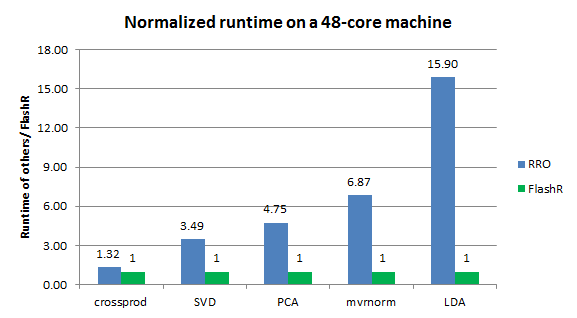
\includegraphics[width=0.5\textwidth]{../../figs/FlashR.vs.RRO.png}
\caption{
Normalized runtime of FlashR vs. Revolution R when executing R implementations
of machine learning primitives on a dataset with one million data points and
1000 features on a large parallel machine with
48 CPU cores. FlashR outperforms Revolution R in all computations. When
the computation gets more complex, the speed advantage of FlashR
over Revolution R gets larger.
}
\label{fig:flashr}
\end{cframed}
\end{figure}

After having efficient matrix operations in the past months, including sparse
matrix multiplication and various dense matrix operations, we integrate all
matrix operations in a single computation framework called FlashR, which
provides both high compatibility with R and efficiency. FlashR now overrides
about 70 R matrix functions in the R
\textit{base} package. As such, we can run existing R code with little
modification or no modification at all. For example, we ported a few R
implementations of machine learning algorithms in the \textit{MASS} package
with little modification. We compare the speed of FlashR against Revolution R,
which is also designed to parallelize and accelerate R code, on a large parallel
machine with 48 CPU cores (Figure \ref{fig:flashr}).
Even for the simple matrix operation such as \textit{crossprod}, FlashR
outperforms Revolution R. As the computation gets more complex, the advantage
of FlashR over Revolution R gets larger. When executing the LDA implementation
(Linear Discriminant Analysis) in the MASS package, FlashR outperforms Revolution R
by over an order of magnitude.

\clearpage

%%%%% Feb

We use FlashR to process the billion-scale datasets to demonstrate its
scalability (Table \ref{tbl:scale}). We use three datasets here: \textit{(i)}
the Criteo dataset has over four billion data points with binary labels
(click vs. no-click), used for advertisement click prediction;
\textit{(ii)} PageGraph is the adjacency matrix of a graph, which has 3.5
billion vertices and 128 billion edges;
\textit{(iii)} PageGraph-32ev are 32 singular vectors that we computed on
the largest connected component of Pagegraph with the tools we built previously.
In these experiments, we run the iterative algorithms
(Logistic regression, k-means and PageRank) on the datasets until they converge.

\begin{table}[h!]
\begin{center}
\caption{The runtime and memory consumption of FlashR on the billion-scale
		datasets on the 48 CPU core machine. The runtime of iterative
		algorithms is measured when the algorithms converge. We run PageRank
		on the PageGraph dataset, run k-means on PageGraph-32ev and the remaining
		algorithms on Criteo.}
\vspace{-10pt}
\footnotesize
\begin{tabular}{|c|c|c|}
\hline
& Runtime (s) & Memory (GB) \\
\hline
Correlation & $91.23$ & $1.5$ \\
\hline
PCA & $136.71$ & $1.5$ \\
\hline
NaiveBayes & $76.55$ & $3$ \\
\hline
LDA & $2280$ & $8$ \\
\hline
Logistic regression & $4154.40$ & $26$ \\
\hline
k-means & $1110.82$ & $28$ \\
\hline
PageRank & $3900$ & $135$ \\
\hline
\end{tabular}
\normalsize
\label{tbl:scale}
\end{center}
\vspace{-10pt}
\end{table}

Even though we process the billion-scale datasets in a single machine (with
48 CPU cores), none of
the algorithms are prohibitively expensive. Simple algorithms, such as
Naive Bayes and PCA, require one or two passes over the datasets and take
only one or two minutes to complete. Logistic regression and k-means take
about $10-20$ iterations to converge. Because the PageRank implementation
uses the power method, it takes $100$ iterations to converge.
Nevertheless, all of the iterative algorithms take about one hour or less.

FlashR scales to datasets with billions of data points easily when running
out of core. Most of the algorithms have negligible memory consumption.
PageRank consumes more memory because the sparse matrix multiplication in
PageRank keeps vectors in memory for semi-external memory computation.
The scalability of FlashR is mainly bound by the capacity of SSDs.
The functional programming
interface generates a new matrix in each matrix operation, which potentially
leads to high memory consumption. Thanks to lazy evaluation and virtual matrices,
FlashR only needs to materialize the small matrices to effectively reduce
memory consumption.

\clearpage
%%%%%% March
We advance FlashR for exploratory analysis on a billion-scale
graph. This includes functions for filtering data points and plotting
histograms and heatmaps on billions of data points. Figure \ref{fig:FlashX}
shows an example of plotting the in-degree histogram of vertices in the page
graph and a heatmap for the distribution of the vertices of the page graph in
a two-dimension space.

\begin{figure}[!h]
\begin{cframed}
\centering
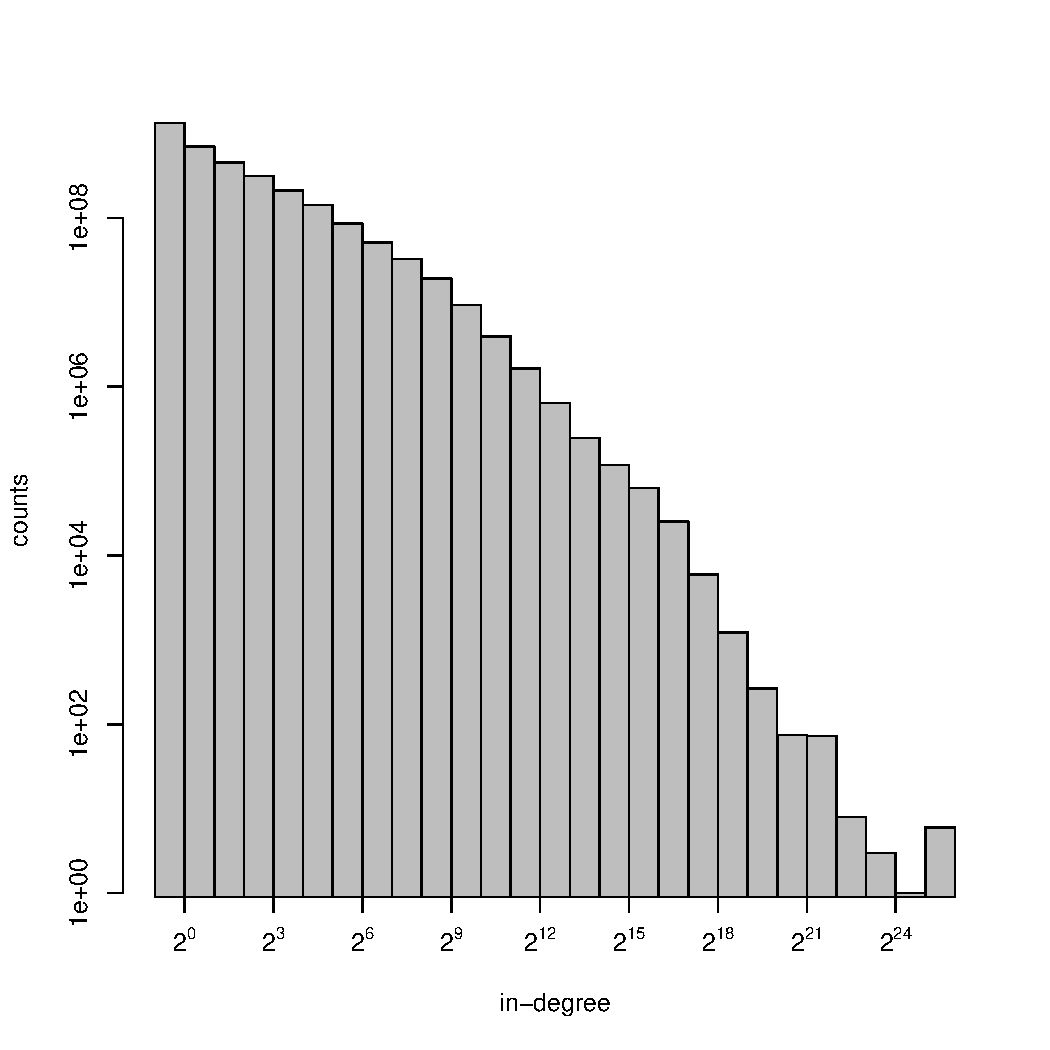
\includegraphics[width=0.4\textwidth]{../../figs/hist-indeg.pdf}
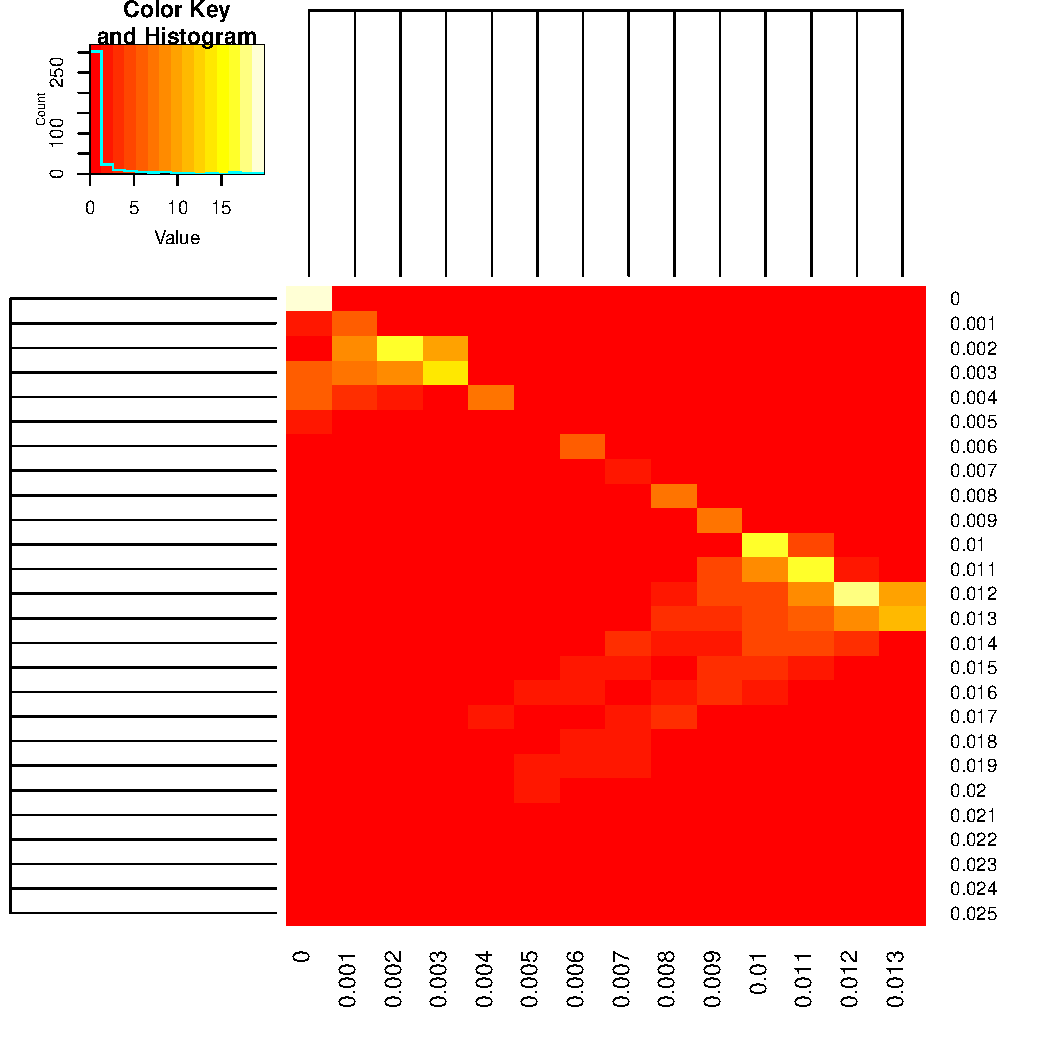
\includegraphics[width=0.4\textwidth]{../../figs/pg_xy_heatmap.pdf}
\caption{Left: the in-degree distribution of the Page graph.
	Right: a heatmap of the distribution of the vertices of the page graph
	in a two-dimension space; the coordinates of the vertices
	in the two-dimension space is determined by the first left and right
	singular vectors.}
\label{fig:FlashX}
\end{cframed}
\end{figure}

\clearpage
\end{document}
